\documentclass[12pt, oneside]{article}   	% use "amsart" instead of "article" for AMSLaTeX format
\usepackage{geometry}                		% See geometry.pdf to learn the layout options. There are lots.
\geometry{a4paper}                   		% ... or a4paper or a5paper or ... 
%\geometry{landscape}                		% Activate for for rotated page geometry
\usepackage[parfill]{parskip}    		% Activate to begin paragraphs with an empty line rather than an indent
\usepackage{graphicx}				% Use pdf, png, jpg, or eps with pdflatex; use eps in DVI mode
\usepackage{amssymb}
\usepackage{epstopdf}				% TeX will automatically convert eps --> pdf in pdflatex		
\usepackage{setspace}
\usepackage{fancyvrb}
\usepackage{float}


\setcounter{secnumdepth}{-1}
\doublespacing
\DefineVerbatimEnvironment{code}{Verbatim}{fontsize=\small}
\newfloat{Pseudo Code}{thp}{lof}


\title{Intelligent Sharing of Occupancy Grids over wireless Adhoc networks on mobile platforms in urban environments}
\author{Matthew Cork}
\date{}							% Activate to display a given date or no date


\begin{document}

\maketitle {}
\newpage
\begin{abstract}
\addcontentsline{toc}{section}{Abstract}
My abstract goes here...
\end{abstract}
\newpage
\renewcommand{\abstractname}{Acknowledgements}
\addcontentsline{toc}{section}{Acknowledgements}
\begin{abstract}
I would like to firstly thank the Mavstar team for the equipment and support to help me in my thesis.\newline
Next I would like to thank my Supervisors Mr Michael Woods and Dr Jose Guivant for their support snd ideas to help me in completion of my Thesis.\newline
I was like to thank Matthew Grosvenor for answering all my networking question to the best of his ability.\newline
Lastly I would like to thank my friends and family for putting up with me while writing the Thesis.
\end{abstract}
\newpage
\renewcommand\contentsname{Table of Contents}
\tableofcontents
\addcontentsline{toc}{section}{Table of Contents}
\newpage
\listoffigures
\addcontentsline{toc}{section}{List of Figures}
\newpage
\section{Chapter 1: Introduction}
\newpage
\section{Chapter 2: Literature Review}
Occupancy Grid's (OG) are an important part of mapping while operating mobile platforms in a ever changing Urban environment. One of the major problems with mapping is the need for multiple devices to map simultaneously. This allows for a fastest and more accurate map to be created but creates a new set of problems. Some of these problems consist of an efficient way to shared the OG to ensure that all the mobile platforms have the same updated map and a lack of infrastructure for wireless communication.

Adhoc networks were designed to eliminate the infrastructure requirements and allow for communication between the mobile platforms without the need of a base station.

Pfingsthorn and Birk  researched into the efficiency of sharing of the Occupancy Grid (OG) through the three following methods; Sending the occupancy grid periodically, sending the cells when they are alter or sending the sensor data used to create the OG. According to their research, the show that the most efficient method to ensure reliability and to eliminate bandwidth hogging.  Each node uses the combination of data sent to generate its own OG map onboard. This method proved to be almost seven times faster than sending the cells as they are modified and over seventy times faster than sending the sections periodically. However the main disadvantage of this method is that all hosts need to have the same data set to have the same occupancy grid. As nodes join and leave they would only get a portion of the data and thus the OG wouldn't be the same. This also would decrease the advantage of having a MAV go offline to explore an area and then synchronise the generated map upon re-entry to the network.

Pham Van's research investigates the issues of bandwidth-hogging and time-sensitivity that is required when streaming video (high volume data) over an adhoc network by proposing a new proactive architecture. The paper analyses the re-transmission time and explains how the new architecture handles the incoming packets. The procedure for handling the incoming packets includes checking if the round trip time  is less than the threshold of delay and if it isn't the packet gets dropped as a smaller path already exist within the node architecture.The packets that have less delay are selected for retransmission to the next node in the sequence. The loss of packets is handles by an NACK which reduces the ACK messages on the bandwidth.

Peak Signal to Noise Ratio is the measurable error between the sent file and the received file. Through experimental testing the paper proves that the Peak Signal to Noise Ratio (PSNR) is a 2.27dB improvement on the conventional case of 32.67dB. The paper clearly presents an architecture that allows the efficient streaming of video in real time. The strength of this approach is that the data is sent over the quickest path and and thus doesn't flood the network. It also handles the loss of packets effectively. The weakness is that as all nodes know if they are part of the quickest route if the structure changes suddenly their is no redundancy for this data to get through. For use in my application we can't assume that the recipient is available and that each node knows the fastest path.

Putta, Prasad, Ravilla, Nath and Chandra outlined the different algorithms used for routing in Mobile Adhoc Networks (MANETS). The paper cover two different reactive algorithms; Adhoc on Demand Distance Vector (AODV) andDynamic Source Routing (DSR), and the main proactive protocol Optimised Link State Routing (OLSR). These algorithms were compared based on the following criteria; Packet Delivery Ratio, Mean end-to-end delay and Routing load. The paper concluded that for all high bandwidth sources proactive protocols (OLSR, etc) allowed for the greatest reliability while for low bandwidth sources, the reactive protocols allow for greatest reliability. Neither reactive protocol proved to be the superior than the other. The paper shows that if the OG was high bandwidth is would be more efficient and reliable to use the proactive protocol. For the control data the more efficient protocol would be either of the reactive protocols. The tests of these protocols however didn't allow for a drastically changing MANET.

Abdel-Hardy and Ward also tested the difference between the proactive protocol (OLSR) and the reactive protocols AODV and Dynamic Manet On Demand (DYMO). They tests include one video stream with five UDP data connections, one video stream with 50 UDP connections and multiple video streams. It the first test it was showed that the DYMO performed better than the AODV while OLSR performed the worse. The second case showed that the AODV was more efficient than the DYMO while both reactive protocols were more efficient than the OLSR. In both these test background data was introduced to measure the effect. For the last test they had multiple video sources transmitting data. This test was consistent with their early two test which showed that for smaller dynamic MANETS the DYMO was more efficient. This paper showed that in a constantly changing MANET the DYMO protocol was the most efficient method of communication for both single and multiple video streams.

\newpage
\section {Chapter 3: Technical Report}
Network communication can be achieved on five main network layers. These layers are the physical, datalink, Network, transport and the application. 
\begin{figure}[H]
\centering
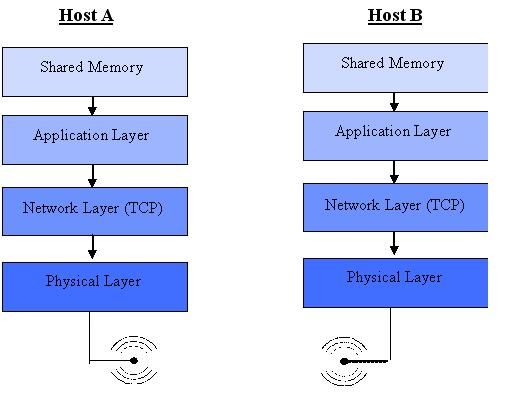
\includegraphics[width=150mm]{Figures/NetworkStructure.jpg}
\caption{Network Levels Structure}
\label{fig:NetworkStructure}
\end{figure}
The transmission of data from the application layer is passed down, through the transport, network, datalink and then finally to the physical link. \newline
The physical link is the only link that has a direct connection to another devices. This base link depends on the method used to connect the devices. This could be via copper, fibre or even wireless. The physical layer sends its data using electrical pulses and waves on the electromagnetic frequency. This is received by other wireless devices for communication. \newline
The link layer sits above the physical layer. This layer is mostly implemented in the Network Interface Card (NIC). The NIC is the onboard hardware that handles the data passed  from the physical layer. The NIC uses the Message Authentication Code (MAC) protocol which gives a unique MAC address for each NIC device. It is responsible for the:
\begin{itemize}
\item Flow control, 
\item Error Detection and Correction,
\item Controlling the Duplexity.
\end{itemize}
The link layer has a buffer has limited size which means that the NIC hardware needs to control the flow from the host to avoid causing the loss of data through data overflow. This is done through two main methods; software and hardware controlled flow. The NIC is in charge of the hardware flow control and will ensure that the data is less than the buffer. The second option is done through software. The only part of the link layer that is implemented in software is the driver which allows the program to interact with the Operating System (OS). This driver controls the the software flow and allows the user to change the setting as needed.  \newline
The error detection and correction is accomplished by using various parity methods. The parity method is given a �parity� value which is can check to see of there is a corruption. By using this method if a corruption has happened the program will be able to detect where the change is and recover from it. These approaches however will not be able to fix major corruption with the data but will be able to detect the change. The cards other main task to to establish wether the user requires a full duplex channel or only a half duplex. If the user only requires one way transmission they can control the duplexity of the channel through the driver. \newline
The two types of communication in the link layer are point to point and broadcasting. The point to point communication requires a single transmitter and a single receiver. The broadcasting communication allows for multiple senders and receivers which causes a problem with over saturation of the bandwidth from any user. The main three methods used to ensure that bandwidth is shared are:
\begin{itemize}
\item Channel Partitioning (FDM and TDM)
\item Random Access
\item Turns based sending.
\end{itemize}
The two methods used in channel partitioning are the Frequency Division Method (FDM) and the Time Division Method (TDM). Both these methods require division of resources to allow for multiple senders and receivers. The FDM divides up the bandwidth frequency with the number of concurrent programs assigning each program a certain the range of the frequency. This then allows the program to use its frequency as it sees fit. The TDM divides the time into frames and assigns each subsection to a different program. Each program is only allowed to transmit during its allocated time. \newline
The random access principle start by transmitting on the full bandwidth. When it detects a collision it will wait a randomly determined time then retransmit all the data. This approach is simple and effective for a small quantity of programs.\newline
The last category is the turn based sending algorithms. There are many different turn based algorithms that are able to be used however the most common and effective are the  ALOHA and SLOTTED ALOHA.
The SLOTTED ALOHA method divides up the link layer frame into segments based on the bits of each frame divide by the full bandwidth on channel. The programs only transmit on the start of their period. This requires the synchronisation of all programs to ensure that no program transmit at the same time.
The ALOHA starts by transmitting on the full bandwidth. When it detects the collision it will determine the wait time based on a probability. This approach doesn�t require any of the programs to be synchronised and still it a simple and effective method of collision avoidance. 
The link layer has many effective means to allow communication between devices as well as error checking/detection built in.\newline
The next layer is the network layer. This layer is implemented entirely in the software and is controlled by the OS. The network layer uses the IP protocol. Due to the dynamic nature of this layer the IP address is often issued by a Dynamic Host Control Protocol (DHCP) Server. However for any system that it fixed, the IP address is often statically defined. This minimises the network overhead for connection and allows for a quicker establishment of communication between the network layers  of different devices. The two main functions of this layer is either forwarding or routing. \newline
Network layer forwarding is the ability for the network layer to determine the correct input to the correct output. This layer is able to sustain many connections simultaneously. When an input in received from one of the connections that need to go to another the connection, the network layer forwarding function is responsible to ensure that the correct input is aligned with the correct output.\newline
The second function of the network layer is the controlling the routing between hosts. Each network layer device has a forwarding table that shows the route to all hosts it has encountered. As the network receives data from new hosts this table is automatically updated by the OS. This data is used by the forwarding function to find the correct output to the host required.\newline
The fourth layer is the transport layer. This layer requires the ports of both the destination and source hosts. This layer uses two different protocols User Datagram Protocol (UDP) and the Transmission Control Protocol (TCP). \newline
The UDP protocol is a connectionless transmission. Due to the lack of connection state, UDP overhead is small. However as the connection can�t be verified, congestion control on this level is almost impossible and this makes the protocol unreliable for data that requires a pattern.\newline
TCP is the most common connection orientated protocol. It is established using a three way handshake. This handshake ensures the reliability of the data transfer. The protocol has three main methods to ensure reliability These are 
\begin{itemize}
\item Stop�n�Wait (SW)
\item Go-Back-N (GBN)
\item Selective Repeat (SR)
\end{itemize}
The TCP protocol can detect and handles congestion in the bandwidth. It does this by throttling the data allowed to be sent by the application layer. The disadvantage of this layer is the limited buffer. To overcome this problem the transport layer provides feedback to the application layer. This requires the application layer to ensure that the data sent is left then the buffer size. The TCP layer is allows for the full duplexity as well.
The SW reliability method is the slowest of the three. When it sends a packet, it waits for acknowledgment that the packet has been received.\newline
The GBN method will send a certain number of packets. It will keep sending the packets in the window until it is acknowledged then will move the window up. This is similar to the SW method however it will send a few packets a once and if nothing goes wrong moves the window by the number of packets.
The SR method also requires a window that keeps track of the the frames sent. As the sender receives an acknowledgement is marks that packet as being received however the windows will only move to the last unacknowledged packet. The packets will only be resent when a timeout period for that packet is reached. This is the quickest method as it only resends packets that timeout.\newline
The last layer is the application layer. This layer is the program that is using the network functions. The are no common protocols for this layer.
The application was chosen for the intelligent sharing of the occupancy grid. This allows for all the safe guards of the lower layers to be used and allowing the program to be written in higher level code with more functionality. 
\newline
Most networking is based on two main types of connection; server-client connections and node based connections. The server client method is the first main type and show in Figure~\ref{fig:serverClient}. This type involves a centralised server that has all the information. The clients then connect to this server and request the information from it. It is usually used when their are few sources of information but many clients. This approach allows for multiple clients to get the same data easily as they know exactly where the source is. This approach fails when a platform needs to be both a client and a source.\newline
\begin{figure}[H]
\centering
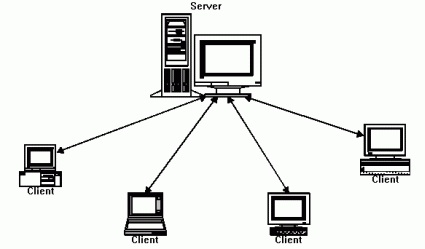
\includegraphics[width=150mm]{Figures/serverClient.jpg}
\caption{Server-Client Connection}
\label{fig:serverClient}
\end{figure}
\begin{figure}[H]
\centering
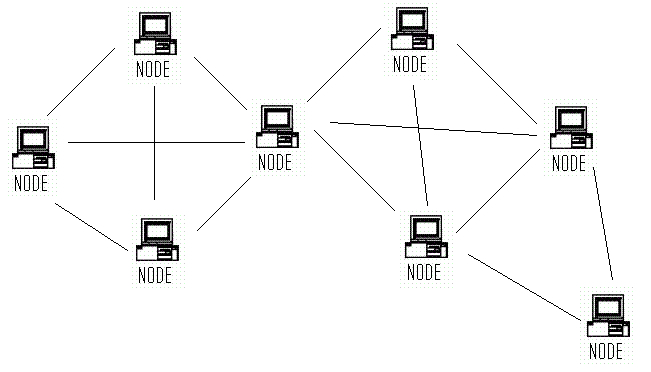
\includegraphics[width=150mm]{Figures/nodeConnection.jpg}
\caption{Node-Node Connection}
\label{fig:node}
\end{figure}
The second main connection is a node to node based communication style as show in Figure~\ref{fig:node}. Node communication is a manager that performs as both a server and client in one program. It requires having a constantly listening port that is used to receive connection requests. Once a request is received then the program establishes connection on another port for communication between the platforms. This approach allows for two way communication between the platforms. The lower network layers handle the connection to ensure that both nodes don�t send at the same time. This connection is used when the both platforms need to communicate information to each other. Node to node connection also performs better than server-client when the number of sources and number of client are similar. The node connection doesn�t always need to be both sending and receiving data but is always capable of the functionality.
\newpage
\section{Chapter 4: The Implementation}
The implementation was separated into two major logical parts to simplify the system and to allow for each section to be developed and tested individually. The modular nature of this approach allows for both parts to be designed to increase the efficiency while keeping separate the different functionality. Another advantage of the modular approach is it allows the shared memory communication to be used as the major inter-process communication (IPC) for the system.
\subsection{Shared Memory Protocol}
The shared memory protocol was designed to allow separate programs to shared data sets between them.  One of the main design criteria for the shared memory communication protocol (SHM Protocol) was to allow multiple sources to publish their data while ensuring that corruption of data was minimised or eliminated. The other main design criteria was the SHM Protocol had to allow multiple receivers to read the latest data and minimise the chance of the data being read being corrupted by another set of data being written over it while it is being read. 
The SHM Protocol starts by creating a file in the platforms local RAM with a particular name (eg "OG"). This "file" is then treated like a normal file allowing for the normal read and write functions to be used. For other people to read/write the data posted they also need to know the "file" name. This libraries have built in optimisations that make writing to memory more efficient then developing my own memory read and write functions. The structure of this "file" is shown in Figure~\ref{fig:shmStructure}
\begin{figure}[H]
\centering
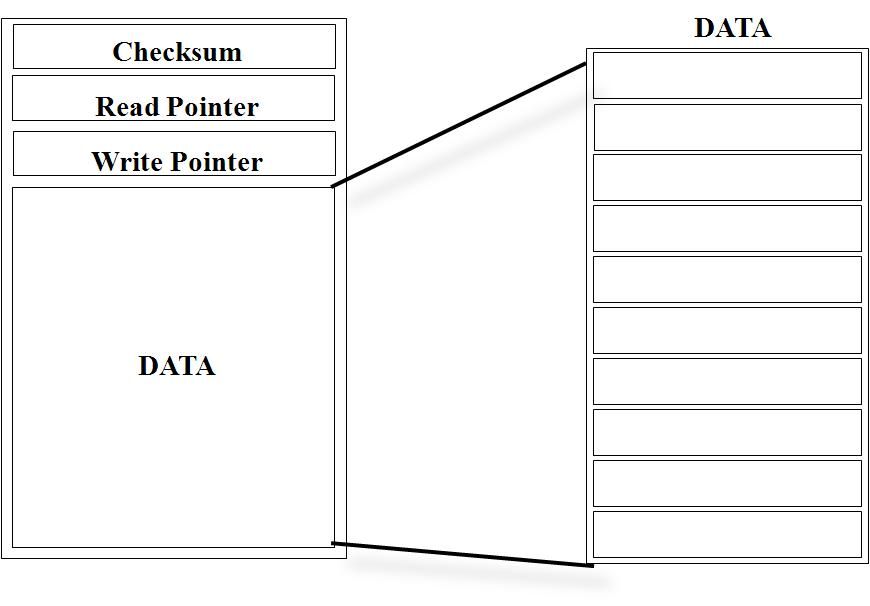
\includegraphics[width=150mm]{Figures/sharedMemory.jpg}
\caption{Shared Memory Structure}
\label{fig:shmStructure}
\end{figure}
The file starts with the checksum. This checksum is used when the a program initially connects to the shared memory file(shm file). The program initially checks to see if the checksum is set to "21289". If this checksum is set that means the file has been initialised by another program. If this value isn't set then the program is responsible to initialise the shared memory and set the initial variables.\newline
The next part of the file is the read and write counter. Both counters are updated when write is called.\newline
The last and biggest part of the structure is the "DATA" segment. This holds the actual data being communicated between the different programs.\newline
One of the major problems with multiple sources reading from or writing to the same data set is the increase chance of corruption. One of the main solutions to this problem is using mutexes or synchronisation locks. Mutexes and synchronisation locks are mutually exclusive locks which prevents multiple people accessing the same file at the same time. This approach is unable to be used as for our purpose we want multiple people to read the data at the same time, while only one person writes at the same time. These approaches also require hardware support to be implemented properly. Due to the above reasons the shared memory protocol needed a different approach to minimise corruption of data. \newline
The solution chosen for the shared memory protocol is using a circular buffer to store the data. The buffer implements an array which can hold ten different instances of the data structure being shared. The right hand side of Figure~\ref{fig:shmStructure} shows the structure of the data segment of the shared memory.
The counters included in the shared memory library (mentioned before) keep track of the next available write element of the array and the current read element. When data is written, the library updates the write counter to the next element of the array while the read counter is updated to the element that has just been written. When read is called, the program requesting data is given a pointer the the last element that was written. When data is written and the read pointer is updated, the old pointer is valid for the next nine writes and only upon the tenth write will the data be overwritten and the chance of corruption would happen. With the buffer size of ten the chance of the data being overwritten and corrupted it greatly reduced. The bigger the buffer is the smaller the chance of corruption, however the greater the buffer the more RAM is taken up in the platforms RAM. Each time read is called the update pointer will be given.\newline
The shared memory protocol is an efficient way to communicate between programs on the platform. It allows multiple sources to write to the common data set without corruption while also allowing multiple sources to read the data. This protocol allows the OG to be shared to the network manager and the OG's sent over the network to this platform to the OG program. The protocol also ensures other programs such as path planning programs can also get the OG for its use. The shared memory protocol is also used as the major IPC communication on the platform for all programs. This is done by changing the name of the file.
\newpage
\subsection{Network}
The network manager was written on the application layer to allow for communication between the various platforms. The program was written as a node style instead of the server-client style as all nodes need to send a receive periodically. This system is superior to the server-client style as once the connection is established the data can be sent both ways across the channel without the need for a second connection. The node is based on the following pseudocode:
\newline
\begin{figure}[htbp]
	\centering
	\begin{code}
	    start listening on port
	    connect to host
	    loop forever
 	    broadcast alive message
	    check for received data
	    if newRecvData {
	   	sync with local OG(using shared memory)
	    }
	    check to see if new data to send
	    if newData {
	  	send New Data
	    }
	\end{code}
	\caption {Pseudo Code: Network Node Implementation}
\end {figure}
The protocol was designed to have a initial listening port that all nodes try to connect to each other on. This allows all nodes to only ever need to try one port number to establish a connection. When a connection is detect, the listen port passes the connection data to another port number. This other port accepts the connection and establishes the two way pipeline to the other node. This approach make the protocol more dynamic and can mean greater number of connections for each node.
After the connection is establish the program then checks to see if new data has been sent over the adhoc network. The TCP connection allows the user to specify a few different options to determine if there is data. These methods are blocking, polling and non-blocking. \newline
Blocking is a method which only returns from the system call when data has been received. This is very useful if data is constantly expected and you can either guarantee the data will be there or if you only want to continue when the data is there. The main disadvantages of this approach is that it will lock up the program and stop it from completing and other tasks until it receives data. \newline
Polling is a way to check the socket connection to see if data has been stored in the buffer since it was last read. This can be a good method when you are expecting data intermittently and constantly opening and closing the connection. However the major disadvantage is that the system call will block if the connection is still open but no data is being sent over it. IT is mainly used when the connection is constantly established and disconnected. \newline
For our approach the only solution that would work is using the non-blocking approach. This approach checks the connection and either returns the data being sent or returns an error code. This major disadvantage with approach is that the node needs to do all the error checking and error-handling itself. The node program checks the return value of the receive system call and handles it appropriately. If data is found, it is then written to the shared memory for the OG implementation to deal with. If the connection has been disconnected from the remote end, then the program would disconnect the socket and wait for another connection. If the connection is still established but no data has been sent through then the nodes skips the writing to shared memory step.

\newpage
\section{Chapter 5: Experiments}
\subsection{Experiment 1 - Shared Memory}
The shared memory implementation is a way to minimise the chance of corruption of the shared buffer using a circular buffer. The corruption is caused by one program over writing the data currently being read. This means the program reading gets partially old data and partially new data which is the corruption. The shared memory experiments are separate into two stages to testing. \newline
\subsubsection{Experiment 1.1 - Benchmarking Shared Memory}
There is currently no benchmark for the size of data shared through the shared memory to determine at what size the corruption is reliable. The first experiment was designed to test structures of different sizes with no multiple data slots for the circular buffer (i.e circular buffer size was one). The purpose of the experiment was to show the size at which corruption first occurs and to develop a benchmark in which data corruption reliably occurs. Using the benchmark allows for future comparison to be made.\newline
The experiment consist of two program accessing the shared memory. The first program was responsible for writing an array of single integers into the shared memory. 
\begin{figure}[htbp]
\centering
\begin{code}
	set integer initial value
	loop forever{
		set all elements of array to integer
		write to share memory
	}
\end{code}
\caption {Pseudo Code: Write program for Shared Memory Testing}
\end{figure}
Two instances of this program are used to write different values to the shared memory.
\newline
The second program was reading the value from shared memory and determining if the data had been corruption. 
\begin{figure}[htbp]
\centering
\begin{code}
	loop forever{
		read from shared memory
		check array for corruption
	}
\end{code}
\caption {Pseudo Code: Read program for Shared Memory Testing}
\end{figure}
\newline
Corruption will be determined by checking the all the values of the array and if the integers aren�t all the same the data was corrupted. The method to obtain the benchmark is outline below.
\newline
\underline {\bf Method}
\begin{enumerate}
\item Change Array Size
\item Run Both Write Programs and Read Program
\item Monitor Output to check if corruption
\item Repeat Steps 1-3 until corruption exists
\end {enumerate}
\newpage
\subsubsection{Experiment 1.2 - Circular Buffer Size}
The second experiment relies on the benchmark obtained in the first experiment to compare the chance of corruption by varying the sizes of the circular buffer. This purpose of the experiment is to prove that the circular buffer can minimise or eliminate the corruption of data and to obtain a reliable circular buffer size for all inter-process communication.\newline
The experiment will start of using an array the size determined in experiment 1.1 as the benchmarking value. The testing procedure will be similar to the method used in experiment 1.1. The circular buffer size will be increase and the tests re-run until the corruption is minimised or eliminated completely.\newline
\underline {\bf Method}
\begin{enumerate}
\item Set Array Size to benchmark size
\item Change Circular Buffer Size
\item Run Both Write Programs and Read Program
\item Monitor Output to check if corruption
\item Repeat Steps 2-4 until corruption disappears
\end {enumerate}
\newpage
\subsubsection{Experiment 1.3 - Circular Buffer Size with Multiple Writers}
The third experiment for the shared memory is to confirm the �safe� recommended value with multiple writers, under heavy computer load and to ensure that the circular buffer values are being updated correctly.\newline
The safe recommended value, for the circular buffer, is chosen to be above the value obtained in experiment 1.2. For this experiment the value 5 was chosen. This should proved to be corruption free as it is higher than the obtained value. This value will then be tested at high load on the computer which will be multiple programs running at the same time. This will allow the experiment to show if increase CPU load and multiple programs writing to the shared memory will result in corruption at the safe value.\newline
A status function was written to allow the read program to read the current values of the read, write counters and the checksum and allowing it to be checked on screen for accuracy.
\newline
\underline {\bf Method}
\begin{enumerate}
\item Set Array Size to benchmark size
\item Set Circular Buffer Size to "safe" size
\item Run Read Program and 10 write programs
\item Monitor Output to check if corruption
\item Monitor Circular Buffer Status to ensure Updating happens 
\end {enumerate}
\newpage
\subsection{Experiment 2 - Network Node Timing}
Experiment 2 was designed to test the end to end timing of the entire approach. This includes the network manager and the shared memory implementations. Timings will be able to compared with other network sharing protocols such as scp. All platforms will have their clocks synced before the testing using the built in linux ntp servers.\newline
Different sizes OG will also be shared over the network, to check to see if there is an optimal size of data being sent. The OG data will be time-stamped by the initial program then written to the shared memory to be shared memory. This changed will be propagated through the network to the next node. The next node will then check the time stamp and display the timing it took for the packet to reach it.\newline
Each data set will consist of twenty changes and the timings will be averaged for that data set to minimise errors created by interference in the bandwidth. The experiment will be repeated with different sizes of OG to determine the ideal size of sending data and allowing a comparison to be made against the same sizes being sent through other sharing programs.\newline
Once the ideal size has been determined this will also give a approximate number of connections that the bandwidth can take without severe flooding of the bandwidth.
\newpage
\section{Chapter 6: Results}
\subsection{Experiment 1 - Shared Memory}
\subsubsection{Experiment 1.1 - Benchmarking Shared Memory}
\begin{figure}[htbp]
\centering
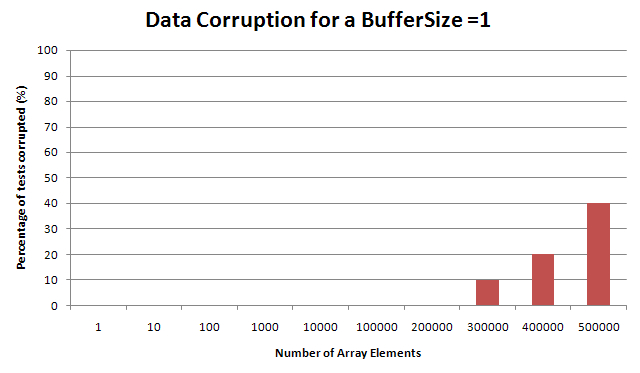
\includegraphics[width=150mm]{Figures/BufferSize1.jpg}
\caption {Results of Experiment 1.1 - Benchmark}
\label{fig:resultBuffer1}
\end{figure}
From Figure~\ref{fig:resultBuffer1}, We can see that corruption began when the the array size has 300000 elements in size. It also showed that in the graph that at 500000 the data corruption was only 40\% of tests. Arrays with number of elements greater than 500000 caused segmentation faults for the program (memory out of bounds). The benchmark determined by the test thus is array size of 500000. This was then used in experiment 1.2.
\newline
\subsubsection{Experiment 1.2 - Circular Buffer Size}
\begin{figure}[htbp]
\centering
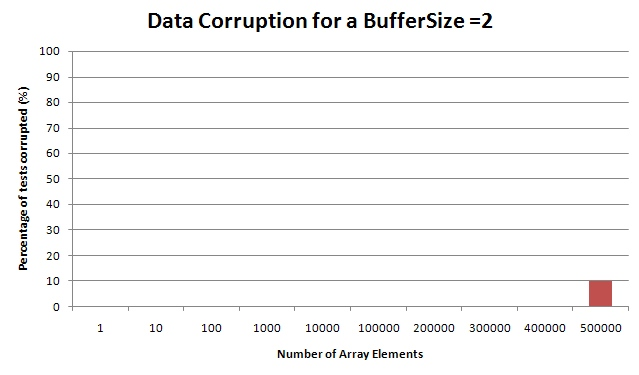
\includegraphics[width=150mm]{Figures/BufferSize2.jpg}
\caption {Results of Experiment 1.2 - Buffer Size = 2}
\label{fig:resultBuffer2}
\end{figure}
The result from Figure~\ref{fig:resultBuffer2} show that the implement of just a circular buffer of two reduced chance of the corruption down to 10\%.
\newline
\begin{figure}[H]
\centering
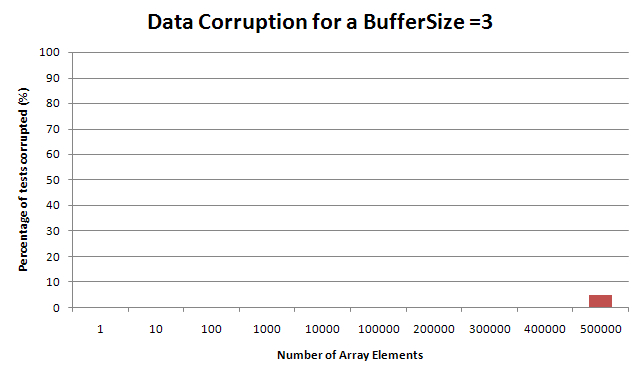
\includegraphics[width=150mm]{Figures/BufferSize3.jpg}
\caption {Results of Experiment 1.2 - Buffer Size = 3}
\label{fig:resultBuffer3}
\end{figure}
The result from Figure~\ref{fig:resultBuffer3} shows that a buffer size of 3 further reduced the chance of corruption of the data. This test showed that only 5\% of the tests showed data corruption.
\newline
\begin{figure}[H]
\centering
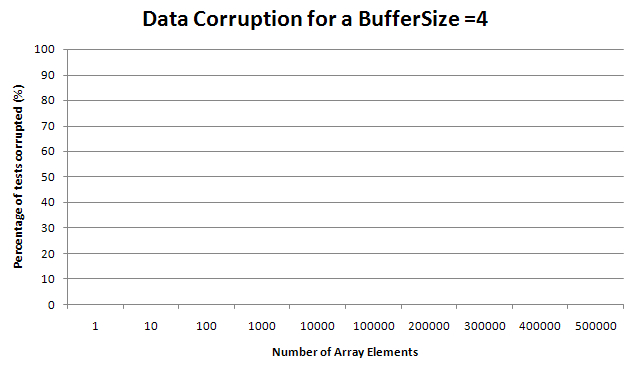
\includegraphics[width=150mm]{Figures/BufferSize4.jpg}
\caption {Results of Experiment 1.2 - Buffer Size = 4}
\label{fig:resultBuffer4}
\end{figure}
Figure~\ref{fig:resultBuffer4} results were obtained with a circular buffer of size 4. The graph shows that data corruption didn't happen for any of the test that were ran.
\newpage
\subsubsection{Experiment 1.3 - Circular Buffer Size with Multiple Writers}
\begin{figure}[H]
\centering
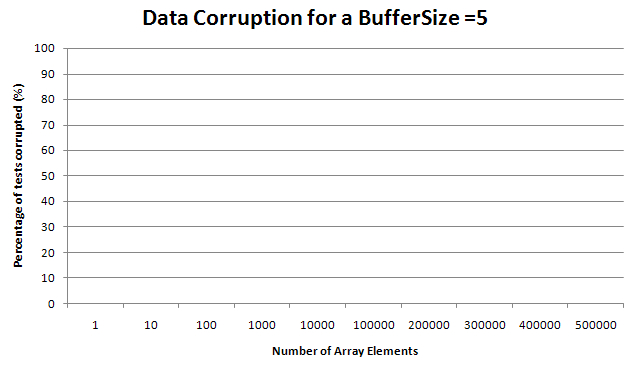
\includegraphics[width=150mm]{Figures/BufferSize5.jpg}
\caption {Results of Experiment 1.3 - Buffer Size = 5}
\label{fig:resultBuffer5}
\end{figure}
The results of this test confirmed that for sizes greater than 4, the data still remains corruption free with more than two writing to the shared memory. 
\begin{figure}[H]
\centering
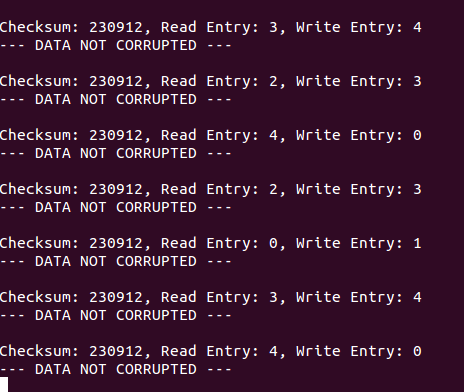
\includegraphics[width=150mm]{Figures/experiment1-3.jpg}
\caption{Results of Experiment 1.3 - Terminal Output}
\label{fig:resultTerminalOutput}
\end{figure}
Figure~\ref{fig:resultTerminalOutput} shows the output from the status function for multiple reads. It shows that the internal values were updated correctly.
\newpage
\subsection{Experiment 2 - Network Node Timing}
\begin{figure}[H]
\centering
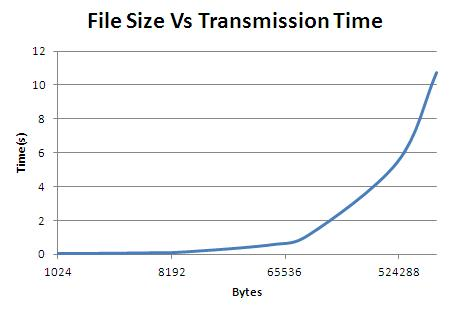
\includegraphics[width=150mm]{Figures/Experiment2Upper.jpg}
\caption{Results of Experiment 2 - Full Graph}
\label{fig:resultExperiment2Full}
\end{figure}
Figure~\ref{fig:resultExperiment2Full} shows that the increase in size has a exponential increase in timing. This was consistent with all sizes between 5kB and 10mB, however above 10mB it was shown that the timing increase proved to be linear with the size increase. Between 0 and 5kB however an interesting graph is produced.\newline
The final timing of 50mB was removed to show greater resolution for the other timings. The timing for 10mB was around 107 seconds..
\begin{figure}[H]
\centering
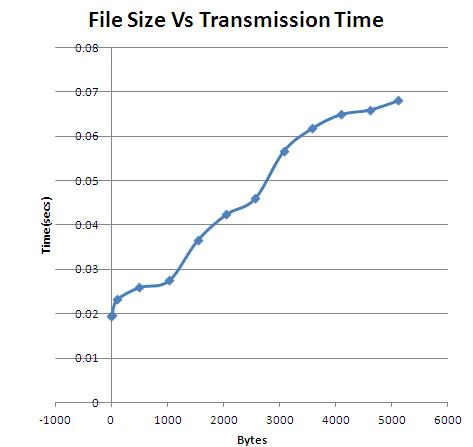
\includegraphics[width=150mm]{Figures/Experiment2Lower.jpg}
\caption{Results of Experiment 2 - Lower Values}
\label{fig:resultExperiment2Low}
\end{figure}
Figure~\ref{fig:resultExperiment2Low} is the section of Figure~\ref{fig:resultExperiment2Full} between 0 and 5kB. Figure~\ref{fig:resultExperiment2Low} shows that graph is a stepping function.
Comparison of SCP was unable to be done due to SCP functions lack of accurate timing.
\newpage
\section{Chapter 7: Discussion}
The implementation shows in the result that both the shared memory and the network manager performed the task required of them, however there were some interesting points in both which will be discussed below.
\subsection{7.1 - Shared Memory}
From Figure~\ref{fig:resultBuffer1} we can see that the corruption doesn�t happen for smaller sizes. This is due to the computer is able to read the shared memory quicker than the program can over write it. The testing was performed on a machine of similar specs to the actual platform. A test was performed on a computer that had greater specs that the platform and that showed that there was no shared memory corruption. The graph also showed that only 40\% of tests were corrupted. This would be mainly caused by the reading happening immediately before another write happens. It would be possible to time the platforms exactly to eliminate corruption however that would require a custom Operating System to controlling all platform timing.(as well as all other OS functions). The greatest number of elements that didn�t cause a segmentation fault was 500000. This was due to an inbuilt restriction on the OS. The total memory usage increased when the circular buffer increased in size so it can be said that memory limit was not reached and thus the maximum size was set by the OS.\newline
Figure~\ref{fig:resultBuffer2} and Figure~\ref{fig:resultBuffer3} showed that as the corruption was minimised as the circular buffer was increased. This shows that the circular buffer implementation was able to eliminate some of the corruption by giving the reading programs more time before the data is overwritten. Figure 8 also shows that data corruption still exists with a circular buffer of size 3. The rate at which the circular buffer decreases wasn�t a proportional amount so it is impossible to work out in advance how big the buffer needs to be for a particular array size. \newline
Figure~\ref{fig:resultBuffer4} shows that corruption didn�t occur at all in the data with a circular buffer of size 4. All these values all are affect by how much the computer is being used for other tasks. To allow for the difference between different computers, and the load on the computer, Experiment 1.3 was tested with a circular buffer of size 5 while having the computer perform multiple instances of the program. Figure~\ref{fig:resultBuffer5} also proves that under a heavier load (multiple programs) the corruption is still eliminated. \newline
Figure~\ref{fig:resultTerminalOutput} in Experiment 1.3 shows that the values inside the shared memory are updating based on each write. The numbers missing in the middle show that all programs are using the same set of pointers and that two people wrote between the reads. It also shows that the read counter is always one previous to the write counter. The experiment was important to ensure that the shared memory was working properly and efficiently and that all programs were using the same set of counters and not either reinitialising each time a program starts or using there own set of counters.\newline
These experimental results show that the data being shared through the shared memory is intelligently and efficiently being communicated between programs and each other or the network manager.
\newpage
\subsection{7.2 - Network Node Timing}
Experiment 2 was conducted by averaging twenty times for the same file size. This was done to help reduce errors created by interference in the wireless range. In most of the tests outliers were found and removed from the average. To establish an outlier, the average was taken and any value more than 20\% greater of less than this value was considered an outlier. The average was then recalculated without this value. This gave a more accurate value for normal timing for each file size. The graphs in the results are without outliers.\newline
Figure~\ref{fig:resultExperiment2Full} contains the values from 1kB up to 5mB. This was necessary as below 1kB was already represented on Figure ~\ref{fig:resultExperiment2Low} and only graphing up to 5mB gave a greater resolution for the other values. Above 10mB the graph tended to be more linear than exponential. \newline
However above 10 mB the values were also much less reliable. \newline
For a file size of 50mB more testing was required as more than half of the timings were over the threshold of an outlier. Most values were around 75\% above or below average with some being over 200\%. With the second set of testing the results were consistent with the first set of testing. This error is to great to include it in the graph results.\newline
Figure~\ref{fig:resultExperiment2Full} shows the overall shape of the curve. As the file size increased the timing was increasing exponentially. This was expected as the data iS increasing with a base of two and each increase will compound by a factor of two. \newline
Figure~\ref{fig:resultExperiment2Low} shows the timings between 1kB and 5kB. These timing show a very unique and complicated pattern. As can be seen from the Figure files sizes under 1kB suggested that the timing was going to plateau. This plateauing indicates a limit in the networking packet size. The shape of the first part of the graph also shows that there is a significant overhead for small packets as the timing increases less the closer the file size gets to 1kB. \newline
From 1kB onwards shows and nonstandard oscillating wave around a 45 degree angle. The curve isn't exactly the same for each period as the first period is larger than the other two. This was an unexpected result as the shape for all other segments were exponential. More research would need to be done to determine if the results are caused by some interference..
\newpage
\section{Chapter 8: Future Work}
All though this approach has been shown to be viable to share the OG data there are ways that the efficiency could be increased. One of the ways to increase the efficiency of network manager would be to translate it to be written on the link layer instead of the application layer. \newline
This approach would eliminate the need for all layers on the networking structure to deal with this data. The link layer would also be able to pass on the data to the next node while simultaneously passing the data up the network stack. This would decrease the propagation time for communication. This would also allow for simplified upper layers of the network stack all the sharing protocol would be handle by the link layer.\newline
The main complication of this approach is the protocol would need to include all the error checking and provide unique identification for each node (a possible implementation could be the MAC address currently used).\newline
Another way that was mention in the discussion was to store non-critical data until the data size is of the optimal size for sending. This will ensure that the bandwidth is used to the greatest efficiency while also ensuring data reaches the other platforms.\newline 
\newline
\newpage
\section{Chapter 9: Conclusion}

\newpage
\section{Appendix}
\end{document}  